\documentclass[a4paper,11pt]{article}
\usepackage[amsbb]{mtpro2}
\usepackage[no-math,cm-default]{fontspec}
\usepackage{xunicode}
\usepackage{xltxtra}
\usepackage{xgreek}
\defaultfontfeatures{Mapping=tex-text,Scale=MatchLowercase}
\setmainfont[Mapping=tex-text,Numbers=Lining,Scale=1.0,
BoldFont={Minion Pro Bold}]{Minion Pro}
\newfontfamily\mpro{Minion Pro}
\usepackage{amsmath}
\usepackage[amsbb]{mtpro2}
\usepackage[left=2.00cm, right=2.00cm, top=2.00cm, bottom=2.00cm]{geometry}
%------TIKZ - ΣΧΗΜΑΤΑ - ΓΡΑΦΙΚΕΣ ΠΑΡΑΣΤΑΣΕΙΣ ----
\usepackage{tikz}
\usepackage{tkz-euclide}
\usetkzobj{all}
\usepackage[framemethod=TikZ]{mdframed}
\usepackage{pgfplots}
\usetkzobj{all}
\usetikzlibrary{calc}
%-----------------------

%-----ΕΙΚΟΝΑ ΔΙΠΛΑ ΑΠΟ ΚΕΙΜΕΝΟ-------
\usepackage{wrapfig}
\newenvironment{WrapText1}[3][r]
{\wrapfigure[#2]{#1}{#3}}
{\endwrapfigure}

\newenvironment{WrapText2}[3][l]
{\wrapfigure[#2]{#1}{#3}}
{\endwrapfigure}

\newcommand{\wrapr}[6]{
\begin{minipage}{\linewidth}\mbox{}\\
\vspace{#1}
\begin{WrapText1}{#2}{#3}
\vspace{#4}#5\end{WrapText1}#6
\end{minipage}}

\newcommand{\wrapl}[6]{
\begin{minipage}{\linewidth}\mbox{}\\
\vspace{#1}
\begin{WrapText2}{#2}{#3}
\vspace{#4}#5\end{WrapText2}#6
\end{minipage}}
%-------------------------------------------
\usepackage{eurosym}
\usepackage{calc}

\renewcommand{\thepart}{\arabic{part}}

\usepackage[explicit]{titlesec}
\usepackage{graphicx}
\usepackage{multicol}
\usepackage{multirow}
\usepackage{enumitem}
\usepackage{tabularx}
\usetikzlibrary{backgrounds}
\usepackage{sectsty}
\sectionfont{\centering}
\usepackage{enumitem}
\setlist[enumerate]{label=\bf{\large \arabic*.}}
\usepackage{adjustbox}
%--------- ΑΓΓΛΙΚΟ ΚΕΙΜΕΝΟ --------------
\newcommand{\eng}[1]{\selectlanguage{english}#1\selectlanguage{greek}}
%----------------------------------------
%------- ΣΥΣΤΗΜΑ -------------------
\usepackage{systeme,regexpatch}
\makeatletter
% change the definition of \sysdelim not to store `\left` and `\right`
\def\sysdelim#1#2{\def\SYS@delim@left{#1}\def\SYS@delim@right{#2}}
\sysdelim\{. % reinitialize

% patch the internal command to use
% \LEFTRIGHT<left delim><right delim>{<system>}
% instead of \left<left delim<system>\right<right delim>
\regexpatchcmd\SYS@systeme@iii
{\cB.\c{SYS@delim@left}(.*)\c{SYS@delim@right}\cE.}
{\c{SYS@MT@LEFTRIGHT}\cB\{\1\cE\}}
{}{}
\def\SYS@MT@LEFTRIGHT{%
\expandafter\expandafter\expandafter\LEFTRIGHT
\expandafter\SYS@delim@left\SYS@delim@right}
\makeatother
\newcommand{\synt}[2]{{\scriptsize \begin{matrix}
\times#1\\\\ \times#2
\end{matrix}}}
%----------------------------------------
%------ ΜΗΚΟΣ ΓΡΑΜΜΗΣ ΚΛΑΣΜΑΤΟΣ ---------
\DeclareRobustCommand{\frac}[3][0pt]{%
{\begingroup\hspace{#1}#2\hspace{#1}\endgroup\over\hspace{#1}#3\hspace{#1}}}
%----------------------------------------
%-------- ΜΑΘΗΜΑΤΙΚΑ ΕΡΓΑΛΕΙΑ ---------
\usepackage{mathtools}
%----------------------

%-------- ΠΙΝΑΚΕΣ ---------
\usepackage{booktabs}
%----------------------
%----- ΥΠΟΛΟΓΙΣΤΗΣ ----------
\usepackage{calculator}
%----------------------------
%------ ΔΙΑΓΩΝΙΟ ΣΕ ΠΙΝΑΚΑ -------
\usepackage{array}
\newcommand\diag[5]{%
\multicolumn{1}{|m{#2}|}{\hskip-\tabcolsep
$\vcenter{\begin{tikzpicture}[baseline=0,anchor=south west,outer sep=0]
\path[use as bounding box] (0,0) rectangle (#2+2\tabcolsep,\baselineskip);
\node[minimum width={#2+2\tabcolsep-\pgflinewidth},
minimum  height=\baselineskip+#3-\pgflinewidth] (box) {};
\draw[line cap=round] (box.north west) -- (box.south east);
\node[anchor=south west,align=left,inner sep=#1] at (box.south west) {#4};
\node[anchor=north east,align=right,inner sep=#1] at (box.north east) {#5};
\end{tikzpicture}}\rule{0pt}{.71\baselineskip+#3-\pgflinewidth}$\hskip-\tabcolsep}}
%---------------------------------

%---- ΟΡΙΖΟΝΤΙΟ - ΚΑΤΑΚΟΡΥΦΟ - ΠΛΑΓΙΟ ΑΓΚΙΣΤΡΟ ------
\newcommand{\orag}[3]{\node at (#1)
{$ \overcbrace{\rule{#2mm}{0mm}}^{{\scriptsize #3}} $};}

\newcommand{\kag}[3]{\node at (#1)
{$ \undercbrace{\rule{#2mm}{0mm}}_{{\scriptsize #3}} $};}

\newcommand{\Pag}[4]{\node[rotate=#1] at (#2)
{$ \overcbrace{\rule{#3mm}{0mm}}^{{\rotatebox{-#1}{\scriptsize$#4$}}}$};}
%-----------------------------------------

%-------- ΤΡΙΓΩΝΟΜΕΤΡΙΚΟΙ ΑΡΙΘΜΟΙ -----------
\newcommand{\hm}[1]{\textrm{ημ}#1}
\newcommand{\syn}[1]{\textrm{συν}#1}
\newcommand{\ef}[1]{\textrm{εφ}#1}
\newcommand{\syf}[1]{\textrm{σφ}#1}
%--------------------------------------------

%--------- ΠΟΣΟΣΤΟ ΤΟΙΣ ΧΙΛΙΟΙΣ ------------
\DeclareRobustCommand{\perthousand}{%
\ifmmode
\text{\textperthousand}%
\else
\textperthousand
\fi}
%------------------------------------------
\usepackage{hhline}
%------------------------------------------
\usepackage{extarrows}
\newcommand{\eq}[1]{\xlongequal{#1}}
%------------------------------------------
%------ ΌΡΙΣΜΑ ----------
\newcommand{\Arg}[8]{
\draw[-latex] (#7,#8)-- ++(#1:#2) node[right=#5]{\footnotesize$#4$};
\draw[fill=black!#6] (#7+0.3+#3,#8) arc (0:#1:0.3+#3) -- (#7,#8);}
%------------------------
\newcommand{\tss}[1]{\textsuperscript{#1}}
\newcommand{\tssL}[1]{\MakeLowercase\textsuperscript{#1}}
\newlist{bhma}{enumerate}{3}
\setlist[bhma]{label=\bf\textit{\arabic*\textsuperscript{o}\;Βήμα :},leftmargin=2cm}
\newlist{rlist}{enumerate}{3}
\setlist[rlist]{itemsep=0mm,label=\roman*.}
\tkzSetUpPoint[size=7,fill=white]
\tikzstyle{pl}=[line width=0.3mm]
\tikzstyle{plm}=[line width=0.4mm]
%----ΣΤΥΛ ΑΣΚΗΣΗΣ ----------
\newcounter{askhsh}[section]
\renewcommand{\theaskhsh}{\bf\thesection.\arabic{askhsh}}   
\newcommand{\Askhsh}[1]{\noindent\refstepcounter{askhsh}\textcolor{black}{{\large \theaskhsh}\hspace{2mm}{\textbf{#1}}}\\}{}
%---------------------------
\newcommand{\unnumsec}[1]{\refstepcounter{section}\section*{#1}}
\renewcommand{\thesection}{\Alph{section}}

\begin{document}

\begin{center}
\textbf{{\large Σπύρος Φρόνιμος}}
\end{center}
\section*{\LARGE ΕΦΑΡΜΟΣΜΕΝΑ ΜΑΘΗΜΑΤΙΚΑ}
\begin{center}
{\normalsize  \bf\today}\mbox{}\\
\vspace{5mm}
\textbf{\large ΣΥΛΛΟΓΗ ΠΡΟΒΛΗΜΑΤΩΝ}
\end{center}
\unnumsec{Α΄ Γυμνασίου}

\unnumsec{Β΄ Γυμνασίου}
\noindent
\Askhsh{Εμβαδά - Πυθαγόρειο Θεώρημα}
\wrapr{-5mm}{10}{3.9cm}{-7mm}{
\begin{tikzpicture}[scale=.7]
\draw  (-4,4) rectangle (0.5,-2);
\draw (-4,1) -- (0.5,1);
\draw  (-1.75,3.2) ellipse (0.6 and 0.6);
\draw[fill=white]  (-3,4) rectangle (-0.5,3);
\draw[fill=white]  (-2.5,4) rectangle (-1,3.5);
\draw  (-1.75,-1.2) ellipse (0.6 and 0.6);
\draw[fill=white]   (-3,-2) rectangle (-0.5,-1);
\draw[fill=white]   (-2.5,-2) rectangle (-1,-1.5);
\draw  (-1.75,1) ellipse (0.6 and 0.6);
\node at (-4.3,4.2){A};
\node at (-4.2,-2.2) {B};
\node at (0.75,-2.2) {$\Gamma$};
\draw (-4,4) -- (0.5,-2);
\end{tikzpicture}}{
Το στάδιο Camp Nou βρίσκεται στην πόλη της Βαρκελώνης στην Ισπανία και είναι έδρα της ποδοσφαιρικής ομάδας FC Barcelona. Το μήκος $ AB $ του ποδοσφαιρικού γηπέδου είναι $ 105m $. Δίνεται γνωστό οτι η διαγώνια απόσταση $ A\varGamma $ ανάμεσα σε δύο απέναντι corner είναι $ 125{,}1m $.
\begin{rlist}
\item Πόσο είναι το πλάτος $ B\varGamma $ του γηπέδου;
\item Να βρεθεί το εμβαδόν που καταλαμβάνει η επιφάνεια του γηπέδου.
\item Αν γνωρίζουμε οτι το κόστος τοποθέτησης του χλοοτάπητα είναι 12\officialeuro\, για κάθε τ.μ. να βρεθεί το συνολικό κόστος τοποθέτησής του.
\end{rlist}}\mbox{}\\\\
\Askhsh{Τριγωνομετρικοί αριθμοί}
Στο κέντρο της πόλης του Παρισιού βρίσκεται ένα από τα πιο σύνθετα αρχιτεκτονικά επιτεύγματα του 19ου αιώνα, ο πύργος του Αϊφελ. Το ύψος του υπερβαίνει τα $300m$ όμως οι τεχνίτες της εποχής δεν είχαν την πολυτέλεια της εξελιγμένης τεχνολογίας που μας επιτρέπει σήμερα να κάνουμε τέτοιους υπολογισμούς με ακρίβεια. 
\begin{center}
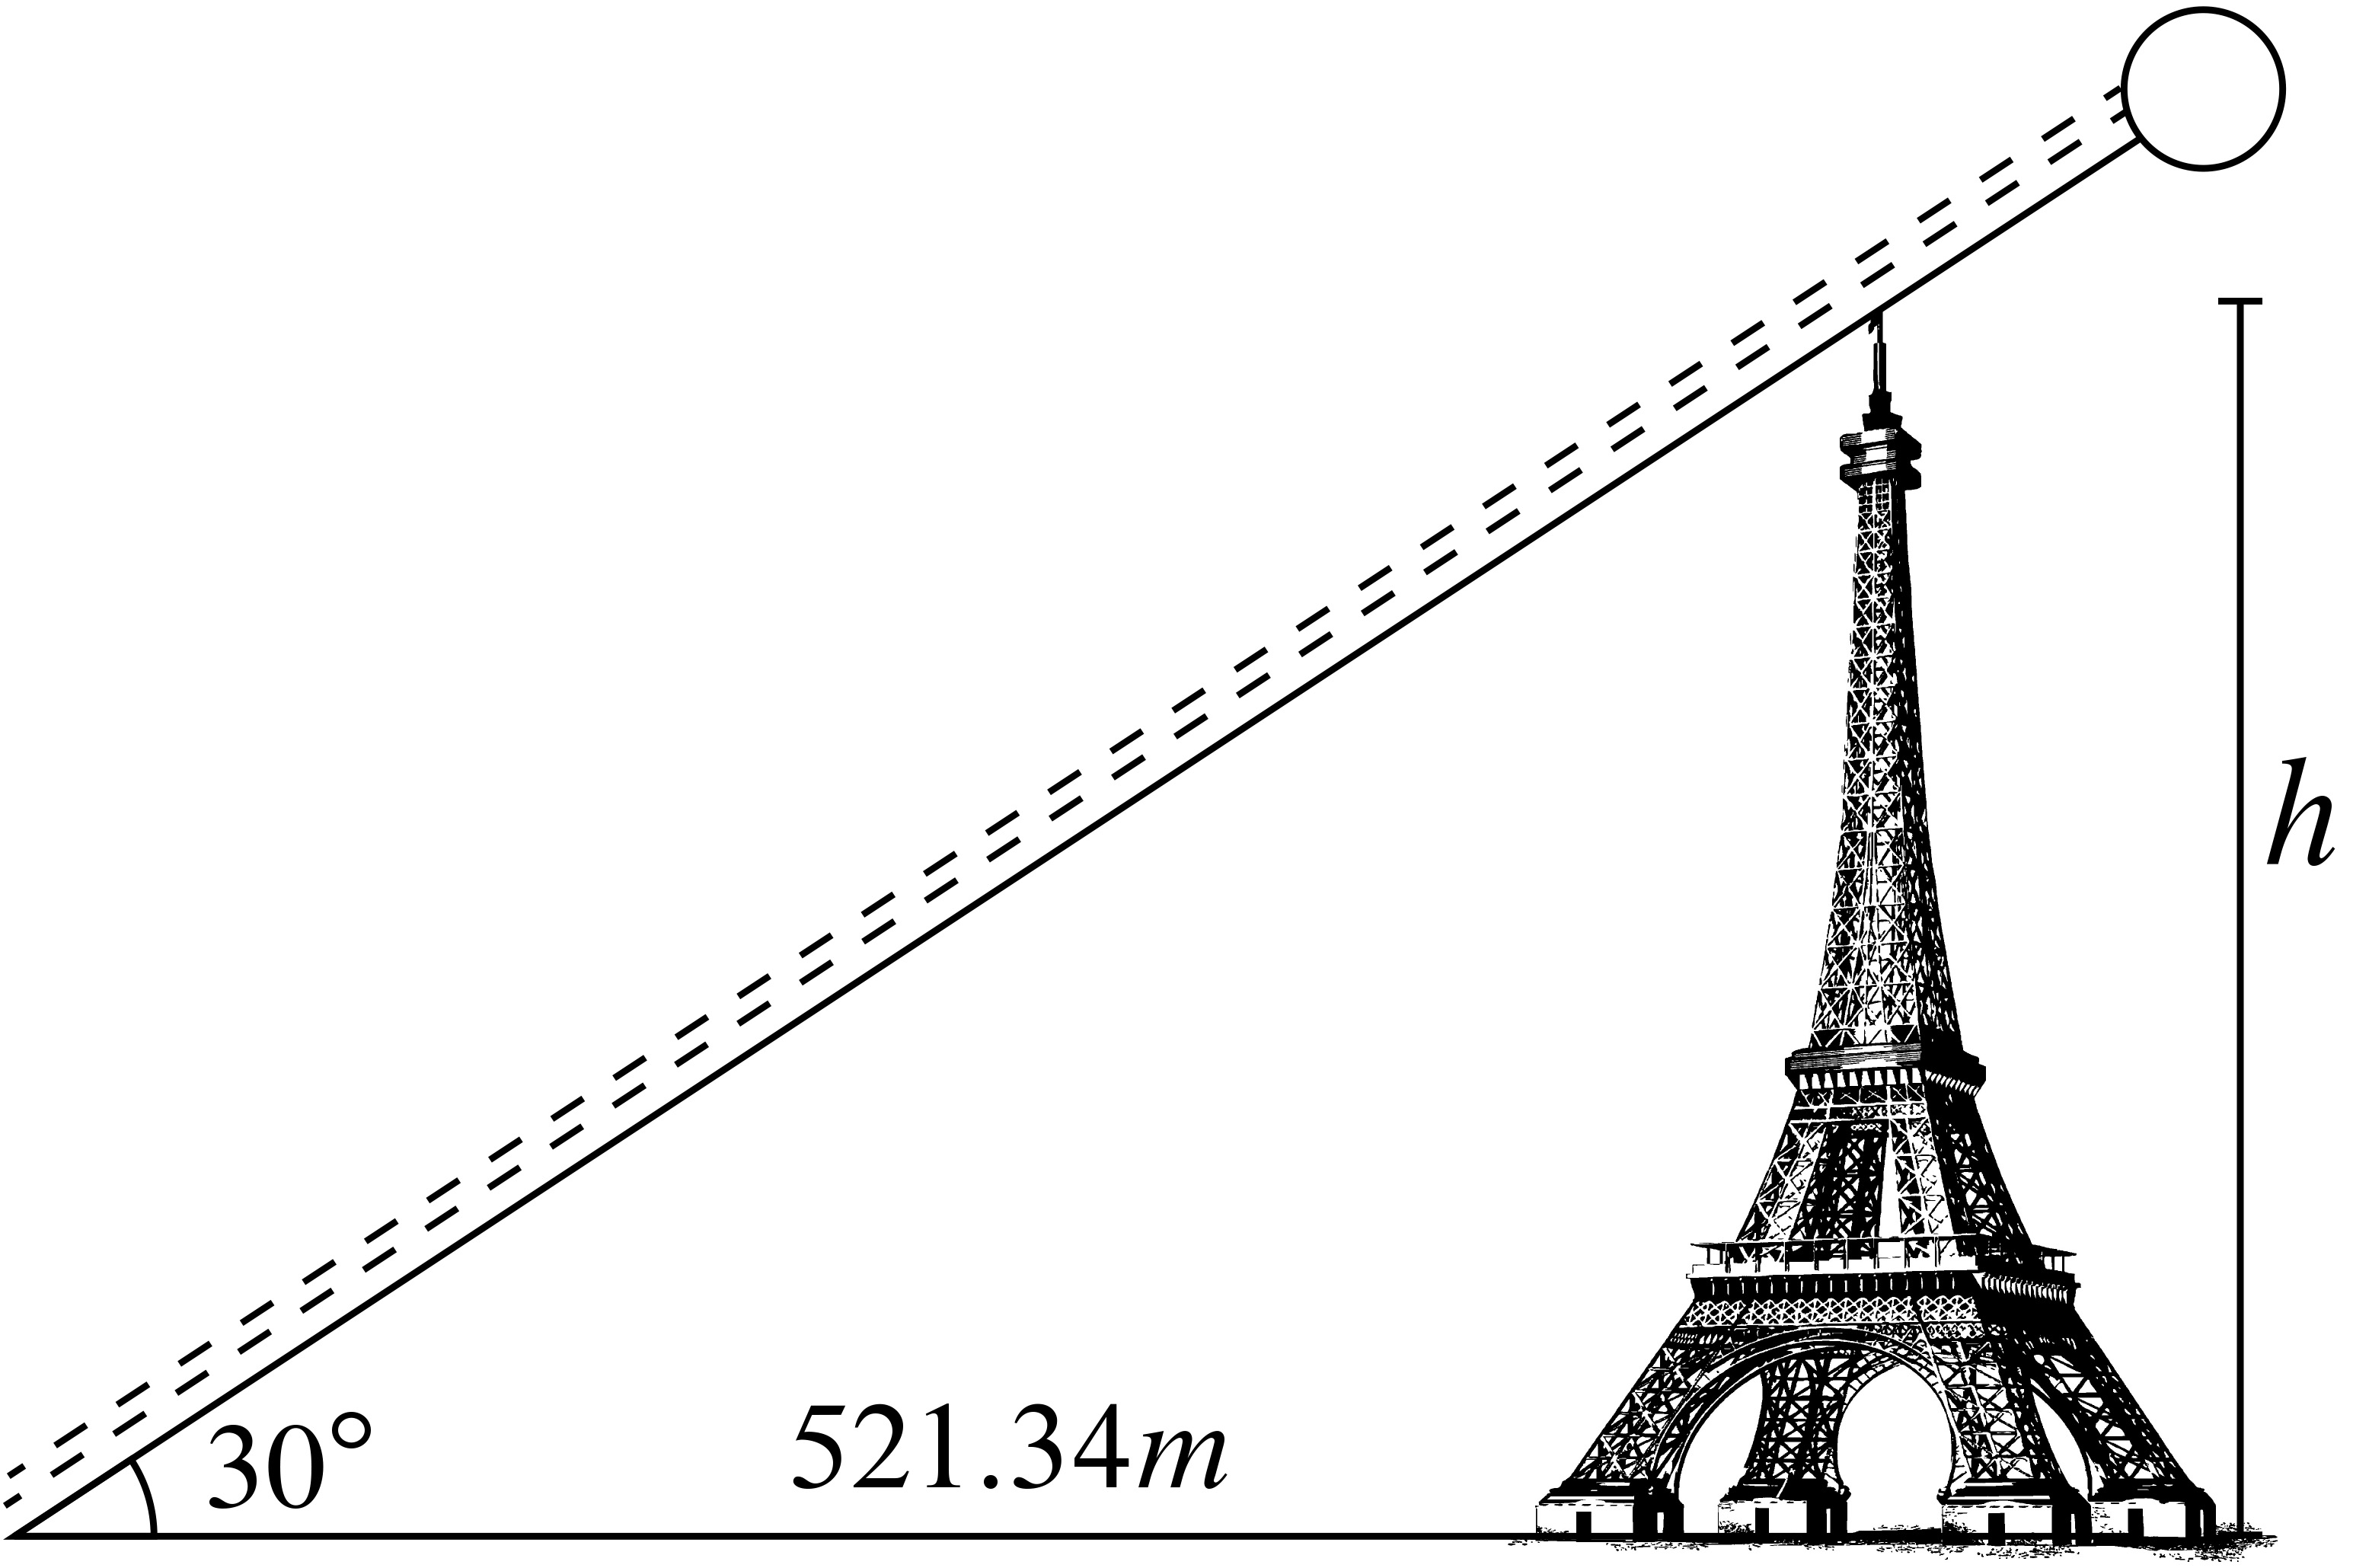
\includegraphics[width=4.95cm, height=3.3cm]{Sxhmata/pyrgos}
\end{center}
Για να υπολογίσουν το ύψος του πύργου θα χρειαστούν τη βοήθεια των αρχαίων Ελλήνων και της Ευκλείδειας Γεωμετρίας. Στις 10 το πρωί ο ήλιος ρίχνει τις ακτίνες του στη Γη με γωνία $ 30^\circ\mkern-1mu $ σε σχέση με το οριζόντιο έδαφος σχηματίζοντας έτσι σκιά μήκους $ 521.34m $ από τη βάση του πύργου. Αν οι τεχνίτες γνωρίζουν ότι $ \ef{30^\circ\mkern-1mu}=\frac{\sqrt{3}}{3} $ τότε δείξτε και σεις πως υπολόγισαν το ύψος του πύργου.
\unnumsec{Γ΄ Γυμνασίου}
\Askhsh{Εξισώσεις 2ου βαθμού}
Οι διαστάσεις ενός δοχείου, σχήματος ορθογωνίου παραλληλεπιπέδου είναι $ x\,cm $, $ x+5\,cm $ και $ 20\,cm $ αντίστοιχα. Ένα άλλο δοχείου ίδιου όγκου κυλινδρικού σχήματος, έχει ύψος $ \frac{30}{\pi}\,cm $ και ακτίνα βάσης $ 10\,cm $.
\begin{rlist}
\item Να βρεθεί η τιμή της μεταβλητής $ x $.
\item Να βρεθεί ο όγκος του 1ου δοχείου.
\end{rlist}
\begin{center}
\begin{tikzpicture}[scale=.5]
\draw[fill=white]  (-3.5,2) node (v2) {} rectangle (-1.5,-1) node (v4) {};
\draw (-3,2.5) node (v1) {} -- (-3.5,2);
\draw (-1,-0.5) node (v5) {} -- (-1.5,-1);
\draw (-1,2.5) node (v3) {} -- (-1.5,2);
\draw (-3,2.5) -- (-1,2.5) -- (-1,-0.5);
\begin{scope}[shift={(0.5,0)}]
\clip (0,-1.1) rectangle (2.5,-0.75);
\draw  (1.25,-0.75) ellipse (1.25 and 0.25);
\end{scope}
\draw  (1.75,2.25) node (v6) {} ellipse (1.25 and 0.25);
\draw (0.5,-0.75) -- (0.5,2.25);
\draw (3,-0.75) -- (3,2.25) node (v7) {};
\draw[|-|] (-3.5,-1.25) -- (-1.5,-1.25);
\draw[|-|] (-1.25,-1.25) -- (-0.75,-0.75);
\draw[|-|] (-0.75,2.5) -- (-0.75,-0.5);
\draw (1.75,2.25) -- (3,2.25);
\node at (-2.5,-1.6) {\scriptsize$x+5$};
\node[rotate={45}] at (-0.75,-1.25) {\scriptsize$x$};
\node at (-0.25,1) {\scriptsize$20$};
\node[fill=white,inner sep=.2mm] at (2.25,2.5) {\scriptsize$10$};
\draw[|-|] (3.25,2.25) -- (3.25,-0.75);
\node at (3.75,0.75) {\scriptsize$\frac{30}{\pi}$};
\end{tikzpicture}
\end{center}
\vspace{-3mm}
Ο όγκος ενός κυλίνδρου δίνεται από τον τύπο $ V=\pi r^2h $ όπου $ r $ είναι η ακτίνα της βάσης και $ h $ το ύψος του.\\\\
\Askhsh{Συστήματα}
Ο μεγάλος υπερτυχερός του λαχείου μόλις κέρδισε $ 4.500.000 $\officialeuro\,  στον πρώτο λαχνό. Τα χρήματα αυτά θα τα παραλάβει από την τράπεζα σε $ 650 $ δεσμίδες των $ 50 $\officialeuro\, και $ 100 $\officialeuro\,. Αν κάθε δεσμίδα περιέχει $ 100 $ χαρτονομίσματα πόσες δεσμίδες από κάθε είδος χαρτονομίσματος θα χρειαστούν;
\setcounter{section}{0}
\unnumsec{Α΄ Λυκείου}
\Askhsh{Πιθανότητες}
Ο καθηγητής των μαθηματικών σε ένα λύκειο πρόκειται να επιλέξει μαθητές από όλες τις τάξεις για να εκπροσωπήσουν το σχολείο στη διεθνή Μαθηματική Ολυμπιάδα του 2015. Θα πρέπει να λάβει υπ όψιν του το αν ο μαθητής είναι αγόρι (α) ή κορίτσι (κ), την τάξη στην οποία πηγαίνει (Α΄, Β΄ ή Γ΄) και το αν έχει συμμετάσχει ξανά (ναι : (ν) ή όχι (ο)) σε οποιονδήποτε διαγωνισμό μαθηματικών.
\begin{rlist}
\item Να βρεθεί ο δειγματικός χώρος του πειράματος.
\item Αν ο καθηγητής επιλέξει τυχαία έναν μαθητή να βρεθεί το ενδεχόμενο
\begin{enumerate}[itemsep=0mm]
\item[Α :] Ο μαθητής να είναι αγόρι.
\item[Β :] Ο μαθητής να ανήκει σε κάποια ομάδα προσανατολισμού και να μην έχει συμμετάσχει ξανά σε διαγωνισμό
\item[Γ :] Ο μαθητής να είναι κορίτσι και να έχει συμμετάσχει ξανά σε μαθηματικό διαγωνισμό.
\end{enumerate}
\item Να υπολογιστούν οι πιθανότητες των παραπάνω ενδεχομένων Α, Β, Γ.
\end{rlist}
\Askhsh{Γεωμετρική πρόοδος}
Κάθε φακός φωτογραφικής μηχανής περιέχει μηχανισμούς ελέγχου της ποσότητας του φωτός που θα εισέλθει μέσα απ' αυτόν. Ο μηχανισμός αυτός ονομάζεται διάφραγμα. Είναι ένα σύνολο από μεταλλικές λεπίδες στο εσωτερικό του, τοποθετημένες με τέτοιο τρόπο ώστε το γεωμετρικό σχήμα του ανοίγματος του διαφράγματος να είναι είτε κανονικό πολύγωνο είτε κύκλος (προσέγγιση κύκλου). Ανοίγοντας ή κλείνοντας το διάφραγμα εισέρχεται περισσότερο ή λιγότερο φως αντίστοιχα. 
\begin{center}
\begin{tabular}{ccc}
$ f/1.4 $ & $ f/2 $ & $ f/2.8 $\\
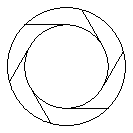
\includegraphics{Sxhmata/1}
& 
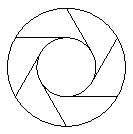
\includegraphics{Sxhmata/2}
 & 
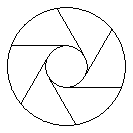
\includegraphics{Sxhmata/3}
 \\ 
\end{tabular} 
\end{center}
Η μονάδα μέτρησης του ανοίγματος ενός διαγράμματος είναι οι "αριθμοί ανοίγματος" η όπως έχει οριστεί διεθνώς τα "f-stops" και συμβολίζονται με $ f/n $. Όσο μεγαλύτερος είναι ο αριθμός αυτός τόσο μικρότερο είναι το άνοιγμα του διαφράγματος όπως φαίνεται στο σχήμα. Το διάφραγμα είναι έτσι κατασκευασμένο ώστε ανάμεσα σε δύο διαδοχικές θέσεις $ f/n $ η ποσότητα φωτός που εισέρχεται από το φακό να είναι δύο φορές μικρότερη από την προηγούμενη. Ο τύπος που δίνει τον αριθμό $ n $ στις διάφορες θέσεις του διαφράγματος είναι 
\[ n=\dfrac{f}{d} \]
όπου $ f $ είναι η εστιακή απόσταση του φακού και $ d $ η διάμετρος του ανοίγματος.
\begin{rlist}
\item Να αποδείξετε ότι οι αριθμοί ανοίγματος του διαφράγματος $ f/n $ αποτελούν όρους γεωμετρικής προόδου $ (F_\nu) $ της οποίας να βρείτε τον γενικό τύπο.
\item Να αποδείξετε ότι τα εμβαδά των ανοιγμάτων του διαφράγματος στις διάφορες θέσεις αποτελούν όρους γεωμετρικής προόδου $ (E_\nu) $ της οποίας να βρείτε τον γενικό τύπο.
\item Να βρεθεί η θέση του διαφράγματος ώστε ο αριθμός ανοίγματος να είναι $ f/5.6 $\footnote{Ο αριθμός $ n $ στις διαβαθμίσεις ενός φακού στρογγυλοποιείται με τέτοιο τρόπο ώστε να αποτελείται από δύο ψηφία.}.
\item Να βρεθεί η θέση του διαφράγματος ώστε το εμβαδόν του ανοίγματος να είναι οχτώ φορές μικρότερο από το αρχικό. Ποιος είναι ο αριθμός $ f/n $ στη θέση αυτή;
\end{rlist}

\unnumsec{Β΄ Λυκείου}
\Askhsh{Συστήματα - Μη γραμμικά συστήματα}
Με βάση το πρότυπο HD Video Standard οι τηλεοράσεις κατασκευάζονται με τέτοιο τρόπο ώστε οι πλευρές τους να έχουν λόγο $ 16:9 $. 
\begin{center}
\begin{tikzpicture}[scale=.8]
\draw[fill=black!10]  (-2,1) rectangle (2,-1.25);
\draw[fill=white]  (-1.75,0.75) rectangle (1.75,-1);
\draw (1.75,0.75) -- (-1.75,-1);
\draw[|-|] (-1.75,-1.5) -- (1.75,-1.5);
\draw[|-|] (2.25,0.75) -- (2.25,-1);
\node at (0,-1.75) {\footnotesize$x$};
\node at (2.5,-.125) {\footnotesize$y$};
\node[rotate={26.5}] at (0.25,-0.25) {\footnotesize διαγώνιος};
\node at (3.5,-0.25) {\footnotesize$\frac{x}{y}=\frac{16}{9}$};
\end{tikzpicture}
\end{center}
Επίσης το μέγεθος μιας τηλεόρασης δίνεται από το μήκος της διαγωνίου της οθόνης δοσμένο σε ίντσες. Μια ίντσα ισούται με $ 2{,}54cm $ $ (1''=2{,}54cm) $. Να βρεθούν οι διαστάσεις της οθόνης μιας τηλεόρασης μεγέθους
\begin{multicols}{3}
\begin{rlist}
\item $ 42'' $
\item $ 49'' $
\item $ 55'' $
\end{rlist}
\end{multicols}
\Askhsh{Κωνικές τομές - Έλλειψη}
Η αίθουσα όπερας του θεάτρου San Carlos στη Λισαβόνα της Πορτογαλίας έχει ελλειπτικό σχήμα (ελλειπτικός κύλινδρος). Αυτό έχει σαν συνέπεια οι θέσεις που βρίσκονται στο ίδιο ύψος να ανήκουν στην ίδια καμπύλη έλλειψης.
\begin{center}
\begin{tikzpicture}[scale=.8]
\pgfmathsetmacro{\a}{3}
\pgfmathsetmacro{\b}{2}
\pgfmathsetmacro{\c}{sqrt(\a^2 - \b^2)}
\begin{scope}
\clip (-2.8,-2.5) rectangle (3.7,2.5);
\draw (0,0) ellipse (1.22*\a cm and 1.22*\b cm);
\end{scope}
\draw (0,0) ellipse (\a cm and \b cm);
\node (E') at (-\c,0){};
\node (E) at (\c,0){};
\tkzLabelPoint[left,xshift=-1mm](E){{\footnotesize Βασιλιάς}}
\tkzLabelPoint[right,xshift=1mm](E'){{\footnotesize Σκηνή}}
\draw[dashed]  (-3.5,1) rectangle (-2,-1);
\draw[dashed]  (2,0.5) rectangle (2.5,-0.5);
\node (M) at ($(0,0)+(80:3 and 2)$) {};
\tkzDrawSegments(E',M M,E)
\tkzLabelPoint[above,xshift=-.5mm,yshift=-.7mm](M){M}
\tkzDrawPoints(E,E',M)
\foreach \x in {0,15,30,45,60,75,90,105,120,135,-15,-30,-45,-60,-75,-90,-105,-120,-135}{
	\node[draw,minimum width=8pt,
	circle,text=white,inner sep=0pt,outer sep=0pt] at ($(0,0)+(\x:3.3 and 2.2)$) {};}
\node[rotate={36}]at (-.4,1){{\footnotesize Ήχος}};
\draw[|-|] (-3,-3) -- (3,-3);
\draw[|-|] (4,2) -- (4,-2);
\node at (0,-3.3) {$50m$};
\node at (4.7,0) {$30m$};
\end{tikzpicture}
\end{center}
Μια απ' αυτές τις ελλείψεις βρίσκεται στο ύψος της σκηνής και του βασιλικού μπαλκονιού. Είναι κατασκευασμένη με τέτοιο τρόπο ώστε η μια εστία της να βρίσκεται στο κέντρο της σκηνής ενώ στην άλλη εστία της βρίσκονται οι βασιλικές θέσεις. Έτσι ο βασιλιάς έχει το προνόμιο να δέχεται τον ήχο αυτούσιο και κρυστάλλινο κατευθείαν στ αυτιά του. Οι διαστάσεις της αίθουσας είναι $ 50m $ και $ 30m $ όπως φαίνονται στο σχήμα.
\begin{rlist}
\item Ποιά είναι η απόσταση που διανύει ο ήχος που ανακλάται πάνω στους τοίχους της αίθουσας και καταλήγει στο βασιλιά;
\item Να βρεθεί η εξίσωση της έλλειψης που ορίζουν οι τοίχοι της αίθουσας στο ύψος της σκηνής.
\item Ποιά είναι η εκκεντρότητα αυτής της έλλειψης;
\item Σε πόση απόσταση βρίσκεται ο βασιλιάς από το κέντρο της σκηνής;
\end{rlist}
\Askhsh{Εμβαδά}
Κάθε φακός φωτογραφικής μηχανής περιέχει μηχανισμούς ελέγχου της ποσότητας του φωτός που θα εισέλθει μέσα απ' αυτόν. Ο μηχανισμός αυτός ονομάζεται διάφραγμα. Είναι ένα σύνολο από μεταλλικές λεπίδες στο εσωτερικό του, τοποθετιμενες με τέτοιο τρόπο ώστε το γεωμετρικό σχήμα του ανοίγματος του διαφράγματος να είναι είτε κανονικό πολύγωνο είτε κύκλος (προσέγγιση κύκλου). Ανοίγοντας ή κλέινοντας το διάφραγμα εισέρχεται περισσότερο ή λιγότερο φως αντίστοιχα. 
\begin{center}
\tikzset{declare function={angleForPoly(\i,\n,\d)=360/\n*\i+\d;
		x_radius              =\pgfkeysvalueof{/tikz/x radius};
		y_radius              =\pgfkeysvalueof{/tikz/y radius};},
	d/.style={circle,fill,outer sep=0pt,inner sep=+0pt,minimum size=+0pt,#1},
	c/.style={insert path={(C) edge[#1,to path={circle[]}] ()}},
	a/.style={insert path={(C)+(left:x_radius+.5cm) edge[#1,<->] +(right:x_radius+.5cm)
			(C)+(  up:y_radius+.5cm) edge[#1,<->] +( down:y_radius+.5cm)}}}
\def\nodeRot{0}
\newcommand*\poly[2][]{%
	\path (0,0) coordinate (C) [rotate/.append code={\def\nodeRot{##1}},#1]
	++ ({angleForPoly(0,#2,0)}:x_radius and y_radius) coordinate[d] (c)
	\foreach \cnt[count=\Cnt from 0] in {0,...,#2} {
		(c) [late options={alias=c'}] 
		coordinate[d] (c) at ({angleForPoly(\cnt,#2,0)}:x_radius and y_radius)
		(c') edge[-] (c)
		\ifnum\Cnt>0 node[anchor={angleForPoly(\Cnt,#2,(180-360/#2)+\nodeRot)},circle]{} \fi};}
\begin{tikzpicture}[>=latex]
\matrix{
\node {$ f/1.4 $}; & \node {$ f/2 $}; &[2mm] \node {$ f/2.8 $}; \\
	\begin{minipage}{2cm}
	\draw circle(3/3);
	\poly[radius=2.45/3,c=dashed]{6}
	\end{minipage} &
	\begin{minipage}{2cm}
	\draw circle(3/3);
	\poly[radius=1.73/3]{6}
	\end{minipage} &[2mm]
	\begin{minipage}{2cm}
	\draw circle(3/3);
	\poly[radius=1.225/3]{6}
	\end{minipage} \\};
\draw(-2.1,-.31)--(-1.3,-.31);
\draw(-2.1,-.31)--(-2.1,-1.3);
\tkzDrawPoint(-2.1,-.31)
\node at (-1.7,-.15){{\scriptsize $R_\nu$}};
\node at (-2.3,-.8){{\scriptsize $R_1$}};
\end{tikzpicture}
\end{center}
Η μονάδα μέτρησης του ανοίγματος ενός διαγράγματος είναι οι "αριθμοί ανοίγματος" η όπως έχει οριστεί διεθνώς τα "f-stops" και συμβολίζονται με $ f/n $. Όσο μεγαλύτερος είναι ο αριθμός αυτός τόσο μικρότερο είναι το άνοιγμα του διαφράγματος όπως φαίνεται στο σχήμα. Οι αριθμοί αυτοί σε έναν απλό φακό αποτελούν όρους γεωμετρικής προόδου με λόγο $ \lambda=\frac{1}{\sqrt{2}}$ πράγμα που σημαίνει οτι η ακτίνα του ανοίγματος ανάμεσα σε δύο διαδοχικούς αριθμούς $ f/n $ είναι $ \sqrt{2} $ φορές μικρότερη. Η πρόοδος που δίνει τους αριθμούς "f-stops" έχει τύπο
\[ F_\nu=f/n=\frac{f/1}{\left(\!\sqrt{2}\right)^{\nu-1} }\;,\;n\approx\left(\!\sqrt{2}\right)^{\nu-1} \]

$ \begin{lgathered}
f : \textrm{Η εστιακή απόσταση του φακού.}\\
f/1 : \textrm{Μέγιστο άνοιγμα διαφράγματος.}\\
n : \textrm{Προσέγγιση της δύναμης }\left(\!\sqrt{2}\right)^{\nu-1}.\\
R_1 : \textrm{Η ακτίνα του μέγιστου ανοίγματος.}\\
R_\nu : \textrm{Η ακτίνα του ανοίγματος σε κάθε θέση } f/n.
\end{lgathered} $\\
Για ένα φακό όπου το άνοιγμα του διαφράγματος έχει σχήμα κανονικού εξαγώνου με μέγιστη ακτίνα $ R_1=32mm $ :
\begin{rlist}
\item Να αποδείξετε οτι το εμβαδόν $ E $ του ανοίγματος του διαφράγματος σε μια τυχαία θέση $ f/n $ είναι διπλάσιο από το αντίστοιχο εμβαδόν $ E' $ της επόμενης θέσης.
\item Nα αποδείξετε οτι τα εμβαδά $ E_\nu $ των ανοιγμάτων διαφράγματος στις διάφορες θέσεις αποτελούν διαδοχικούς όρους γεωμετρικής προόδου της οποίας να βρείτε τον γενικό τύπο.
\item Nα υπολογίσετε τα εμβαδά $ E_2,E_5 $ και $E_8$ (αντιστοιχούν στις θέσεις $ f/1.4, f/4 $ και $ f/11 $.)
\end{rlist}
\unnumsec{Γ΄ Λυκείου}
\Askhsh{Ακρότατα}
Ένα εργοστάσιο κονσερβοποιίας κατασκευάζει κυλινδρικές κονσέρβες με ύψος $ \mathrm{h}\,cm $ και ακτίνας βάσης $ \mathrm{r}\,cm $. Ο όγκος κάθε κονσέρβας είναι $ 500ml $ και είναι κατασκευασμένη από αλουμίνιο. Γνωρίζουμε επίσης οτι ο όγκος $ V $ και το εμβαδόν $ E $ ενός κυλίνδρου δίνονται αντίστοιχα από τους τύπους \[ V=\pi r^2h\;\;,\;\;E=2\pi rh+2\pi r^2 \]
\begin{rlist}
\item Να εκφραστεί το ύψος $ \mathrm{h} $ της κονσέρβας ως συνάρτηση της ακτίνας $ \mathrm{r} $ της βάσης της.
\item Να εκφραστεί το εμβαδόν $ E $ της κονσέρβας ως συνάρτηση της ακτίνας $ \mathrm{r} $ της βάσης της.
\item Να βρεθεί πόσο πρέπει να είναι η ακτίνα της βάσης ώστε το εμβαδόν τους, και κατά συνέπεια το κόστος παραγωγής, να είναι το ελάχιστο.
\item Για την τιμή της ακτίνας η οποία δίνει το ελάχιστο εμβαδόν να βρεθεί το ύψος $ \mathrm{h} $, το εμβαδόν $ E $ της κονσέρβας καθώς και το κόστος παραγωγής 500.000 κονσερβών αν ξέρουμε ότι η αξία των φύλλων αλουμινίου που χρειάζονται για να κατασκευαστούν οι κονσέρβες είναι 20\officialeuro\, ανα τ.μ.
\end{rlist}

\end{document}